\documentclass[12pt]{article}
\usepackage{makecell}
\usepackage{hyphenat}
\usepackage[utf8]{vietnam}
\usepackage[vietnamese=nohyphenation]{hyphsubst}
\usepackage[vietnamese]{babel}
\usepackage[table,dvipsnames]{xcolor} % Required for row coloring
\usepackage{booktabs} % Required for nicer horizontal lines
\usepackage{ragged2e}
\usepackage{caption}
\usepackage{subcaption}
\usepackage{float}
\usepackage{amsmath,amssymb,amsfonts}
\usepackage{graphicx}
\usepackage{adjustbox}
\usepackage{multicol}
\usepackage[inline,shortlabels]{enumitem}
\usepackage{setspace}
\usepackage{longtable}
\usepackage{bm} 
\usepackage[inkscapelatex=false]{svg}
\usepackage{titling}
\usepackage{tabularx}
\usepackage[T1]{fontenc}
\usepackage{lmodern,mathrsfs}
% \usepackage[draft]{hyperref}
\usepackage{hyperref}
\usepackage{xparse}
\usepackage{fontawesome5}
\usepackage[most]{tcolorbox}
\usepackage{tikz}
\usepackage[framemethod=TikZ]{mdframed}
\usetikzlibrary{matrix, fit, shadows, positioning, arrows.meta, calc, shapes.geometric, backgrounds, shapes.symbols}
\usepackage{paracol}
\usepackage{bbm}
\usepackage{pgfplots}
\usepackage{siunitx}
\usepackage{multirow}
%  biblatex (thay cho IEEEtran.bst) ------------------------------------
\usepackage[
    backend=bibtex,
    style=ieee,
    citestyle=numeric-comp,
    maxnames=1,     % chỉ hiển thị 1 tên tác giả, phần còn lại thành ``et al."
    minnames=1,
    uniquelist=false,
    hyperref=false
]{biblatex}
\usepackage{forest}
% \addbibresource{references.bib} % bỏ trống vì tài liệu này chưa dùng citation
\DefineBibliographyStrings{english}{
  andothers = {et\addabbrvspace al\adddot}
}
\AtBeginBibliography{\selectlanguage{english}}

% -----------------------------------------------------------------
\AtBeginDocument{\renewcommand\refname{}}

\usepackage[toc,page]{appendix}
\renewcommand{\appendixtocname}{Phụ lục}      
\renewcommand{\appendixpagename}{Phụ lục}

\usepackage{xurl}
\setlength{\headheight}{14.5pt}
\setlength{\topmargin}{-.5in} \setlength{\textheight}{9.25in}
\setlength{\oddsidemargin}{-0.1in} \setlength{\textwidth}{6.8in}

\usepackage{tocloft}
\renewcommand{\cfttoctitlefont}{\Huge\bfseries}
\setlength{\cftaftertoctitleskip}{2em}
\setlength{\cftbeforesubsecskip}{7pt} % giãn cách subitem mục lục
\renewcommand{\cftsecleader}{\cftdotfill{\cftdotsep}}
\setlength{\cftsecnumwidth}{3em}
\renewcommand{\cftsecaftersnum}{\quad}
\renewcommand{\cftsubsecleader}{\cftdotfill{\cftdotsep}}
\setlength{\cftsubsecnumwidth}{4em}
\renewcommand{\cftsubsecaftersnum}{\quad}
\renewcommand{\cftsubsubsecleader}{\cftdotfill{\cftdotsep}}
\setlength   {\cftsubsubsecnumwidth}{5em}  
\renewcommand{\cftsubsubsecaftersnum}{\quad}

\PassOptionsToPackage{vietnamese.licr}{babel}
\usepackage{../../latex/styles/vipythonhighlight}
\usepackage{../../latex/styles/tvietlistings}
\newcounter{mycounter}
\newcommand\showmycounter{\stepcounter{mycounter}\themycounter}
\usepackage{lipsum}
\newcommand\showlips{\stepcounter{mycounter}\lipsum[\value{mycounter}]}

%--------------------------------------------------------------------
\usepackage{framed}
\usepackage{fancyhdr}
\usepackage{upquote}
\usepackage{listings}	 

\usepackage[toc, nonumberlist, style=super]{glossaries}
\makenoidxglossaries

\newglossarystyle{clean3col}{%
    % 1) Table layout: 3 columns
    \renewenvironment{theglossary}%
    {%
      \begin{longtable}{@{}
        >{\setlength{\parindent}{0pt}\RaggedRight\arraybackslash}p{0.2\linewidth}
        >{\setlength{\parindent}{0pt}\RaggedRight\arraybackslash}p{0.23\linewidth}
        >{\setlength{\parindent}{0pt}\RaggedRight\arraybackslash}p{0.52\linewidth}
      @{}}%
    }%
    {\end{longtable}}%

    % 2) Header row
    \renewcommand{\glossaryheader}{%
        \bfseries Thuật ngữ &
        \bfseries Tạm dịch &
        \bfseries Mô tả \\
        \midrule
        \endhead
    }%

    % 3) Each entry row
    \renewcommand{\glossentry}[2]{%
        \itshape \glstarget{##1}{\glossentryname{##1}} &
        \glsentryuseri{##1} &
        \glossentrydesc{##1} \\
        \addlinespace[6pt]
    }%
}


% Color --------------------------------------------------------------------
\usepackage{epigraph}
\usepackage{titlesec}

\definecolor{codebackground}{RGB}{250, 250, 250}
\definecolor{codecomment}{RGB}{34, 139, 34}
\definecolor{codekeyword}{RGB}{0, 0, 255}
\definecolor{codestring}{RGB}{255, 0, 0}
\definecolor{codeidentifier}{RGB}{0, 0, 0}
\definecolor{codelinenumbers}{RGB}{90, 90, 90}

\definecolor{codegreen}{rgb}{0,0.6,0}
\definecolor{codegray}{rgb}{0.5,0.5,0.5}
\definecolor{codepurple}{rgb}{0.58,0,0.82}
\definecolor{backcolour}{rgb}{0.95,0.95,0.92}

\definecolor{aivnGreen}{RGB}{52,79,30}  
\definecolor{aivnCodeOutputColor}{RGB}{11,83,148}  
\definecolor{captiongray}{gray}{0.15} 
\definecolor{captionbg}{RGB}{250,250,250}

\definecolor{foldercolor}{RGB}{0, 102, 204}
\definecolor{filecolor}{RGB}{104, 104, 104}
\definecolor{scriptcolor}{RGB}{180, 50, 50}
\definecolor{pythoncolor}{RGB}{0, 128, 128}

% --- Extra Brand colors for the table ---
\definecolor{brandIndigo}{HTML}{333D91} 
\definecolor{rowLavender}{HTML}{EEECFA}
\setlength{\parskip}{0.3em}

% Table
\newtcolorbox{captionbelowboxaivn}{
    colback=aivnGreen,
    colframe=aivnGreen,
    boxrule=0pt,
    arc=4pt,
    left=4pt,
    right=4pt,
    top=2pt,
    bottom=2pt,
    width=\linewidth,
    boxsep=4pt,
    halign=center,
    % fontupper=\bfseries\color{white}
    fontupper=\color{white}
}

% Figure
\newtcolorbox{figurecardcaptionaivn}{
  colback=aivnGreen,        % Màu nền (background color)
  colframe=aivnGreen,       % Màu viền box (border color)
  boxrule=0pt,              % Độ dày viền box (0pt = không viền)
  arc=2pt,                  % Độ bo góc (2pt là bo nhẹ, tăng để bo tròn hơn)
  top=3pt,                  % Padding phía trên nội dung
  bottom=3pt,               % Padding phía dưới nội dung
  left=10pt,                % Padding bên trái
  right=10pt,               % Padding bên phải
  width=\linewidth,         % Chiều rộng bằng toàn bộ dòng
  fontupper=\small\fontsize{11pt}{13pt}\selectfont\color{white} 
}

% Tạo counter riêng
\newcounter{hinh}
% Định nghĩa macro caption Hình
\newcommand{\capfig}[1]{%
  \refstepcounter{hinh}%
  % \textbf{Hình~\thehinh:}~#1
    Hình~\thehinh:~#1
}

\newtcolorbox{figurecaptionmodern}{
  colback=captionbg,
  colframe=aivnGreen,
  boxrule=1.5pt,
  bottomrule=2pt,  
  toptitle=0pt,
  bottomtitle=0pt,
  left=6pt,
  right=6pt,
  top=4pt,
  bottom=2pt,
  width=\linewidth,
  fontupper=\small\fontsize{11pt}{13pt}\selectfont\color{black},
  halign=center
}

% Code Block -----------------------------------------------------------------
\newtcolorbox{aivncodebox}[1][]{%
  enhanced,
  colback=gray!10,
  colframe=aivnGreen,
  coltitle=white,
  colbacktitle=aivnGreen,
  title=#1,
  fonttitle=\bfseries\sffamily,
  listing only,
  breakable,
  listing engine=listings,
  listing options={
    language=Python,
    basicstyle=\ttfamily\footnotesize,
    commentstyle=\color{ForestGreen},
    keywordstyle=\color{blue},
    stringstyle=\color{red!70!black},
    numbers=left, upquote=true,
    numberstyle=\tiny\color{gray},
    numbersep=5pt,
    breaklines=true,
    showstringspaces=false,
    xleftmargin=1.5em,
    framexleftmargin=1.5em
  }
}

% Code Output Block -----------------------------------------------------------------
\newtcolorbox{aivnCodeOutput}[1][]{%
  enhanced,
  colback=gray!10,
  colframe=aivnCodeOutputColor,
  coltitle=white,
  colbacktitle=aivnCodeOutputColor,
  title=#1,
  fonttitle=\bfseries\sffamily,
  listing only,
  breakable,
  listing engine=listings,
  listing options={
    language=Python,
    basicstyle=\ttfamily\footnotesize,
    commentstyle=\color{ForestGreen},
    keywordstyle=\color{blue},
    stringstyle=\color{red!70!black},
    numbers=left,
    numberstyle=\tiny\color{gray},
    numbersep=5pt,
    breaklines=true,
    showstringspaces=false,
    xleftmargin=1.5em,
    framexleftmargin=1.5em
  }
}

% Last argument allows more tcolorbox options to be added

% --- SQL code box ------------------------------------------------------------
\lstdefinestyle{sqlstyle}{
    backgroundcolor=\color{codebackground},
    keywordstyle=\color{blue}\bfseries,
    stringstyle=\color{red!70!black},
    commentstyle=\color{ForestGreen}\itshape,
    basicstyle=\ttfamily\footnotesize,
    columns=fullflexible,
    keepspaces=true,
    numbers=left,
    numberstyle=\tiny\color{gray},
    numbersep=5pt,
    breaklines=true,
    showstringspaces=false,
    upquote=true,
    xleftmargin=1.5em,
    framexleftmargin=1.5em
}

\newtcblisting{aivnsqlbox}[1][]{%
  enhanced,
  colback=gray!10,
  colframe=aivnGreen,
  coltitle=white,
  colbacktitle=aivnGreen,
  title=#1,
  fonttitle=\bfseries\sffamily,
  listing only,
  breakable,
  listing engine=listings,
  listing options={language=SQL, style=sqlstyle}
}

% --- Plain text / config (YAML, Jinja) code box ------------------------------
\lstdefinestyle{plainstyle}{
    backgroundcolor=\color{codebackground},
    basicstyle=\ttfamily\footnotesize,
    columns=fullflexible,
    keepspaces=true,
    numbers=left,
    numberstyle=\tiny\color{gray},
    numbersep=5pt,
    breaklines=true,
    showstringspaces=false,
    upquote=true,
    xleftmargin=1.5em,
    framexleftmargin=1.5em
}

\newtcblisting{aivnplainbox}[1][]{%
  enhanced,
  colback=gray!10,
  colframe=aivnCodeOutputColor,
  coltitle=white,
  colbacktitle=aivnCodeOutputColor,
  title=#1,
  fonttitle=\bfseries\sffamily,
  listing only,
  breakable,
  listing engine=listings,
  listing options={language={}, style=plainstyle}
}

% --- Placeholder cho sơ đồ cần vẽ sau ----------------------------------------
\newcommand{\diagramplaceholder}[2][5.5cm]{%
  \begin{center}
  \begin{tcolorbox}[enhanced, breakable,
      colback=gray!4, colframe=gray!60, boxrule=0.8pt, arc=4pt,
      width=\linewidth, height=#2, valign=center, halign=center]
    {\color{gray}\sffamily\faImage\hspace{1em}\textbf{[PLACEHOLDER --- Sơ đồ]}}\\[8pt]
    {\color{gray}\sffamily\itshape #1}
  \end{tcolorbox}
  \end{center}
}

% --- Guideline/Tip box ---
\newtcolorbox{guidelinebox}[2][]{
    enhanced, colback=yellow!10!white, colframe=orange!90!black, boxrule=1pt, arc=4pt,
    fonttitle=\bfseries, attach boxed title to top left={yshift=-2mm, xshift=3mm},
    colbacktitle=orange!90!black, coltitle=white,
    title=\faLightbulb\hspace{1mm} #2, #1
}

\newtcolorbox{notebox}[1][]{
  enhanced,  colback=yellow!10, colframe=orange!80, boxrule=1pt, 
  arc=4pt, fontupper=\small, attach boxed title to top left={yshift=-2mm, xshift=3mm},
  colbacktitle=orange!80,  coltitle=white, fonttitle=\bfseries,  
  title=\faInfoCircle~\textbf{Lưu ý},  #1
}

\newtcolorbox{infobox}[1]{%
    enhanced, 
    breakable, 
    colback=green!3, 
    colframe=green!3, 
    arc=5pt,
    borderline west={3pt}{0pt}{aivnGreen},
    attach boxed title to top left={ 
        yshift*=-\tcboxedtitleheight/2, 
        xshift=-0.1em 
    },
    colbacktitle=aivnGreen, %
    coltitle=white, 
    fonttitle=\bfseries, 
    boxed title style={ 
        arc=4pt, 
        top=2pt, 
        bottom=2pt,
        left=8pt,
        right=8pt,
    },
    title={\faInfoCircle\quad #1}
}
\newtcolorbox{examplebox}[1]{%
    enhanced,
    breakable,
    colback=brandIndigo!5,      
    colframe=brandIndigo!5,     
    arc=5pt,
    borderline west={3pt}{0pt}{brandIndigo}, 
    attach boxed title to top left={
        yshift*=-\tcboxedtitleheight/2,
        xshift=-0.1em
    },
    colbacktitle=brandIndigo,   
    coltitle=white,
    fonttitle=\bfseries,
    boxed title style={
        arc=4pt,
        top=2pt,
        bottom=2pt,
        left=8pt,
        right=8pt,
    },
    title={\faLightbulb\quad #1} 
}
% Prompt Block ---------------------------------------------------------------
\definecolor{promptBlue}{HTML}{2F5D8C}
\definecolor{promptBg}{HTML}{F6F9FC}
\definecolor{promptBorder}{HTML}{B7C9DC}

% Dùng cho prompt đã viết theo cú pháp LaTeX bình thường
\newtcolorbox{promptbox}[1][Prompt]{%
    enhanced,
    breakable,
    colback=promptBg,
    colframe=promptBorder,
    coltitle=white,
    colbacktitle=promptBlue,
    fonttitle=\bfseries\sffamily,
    title={#1},
    boxrule=0.8pt,
    arc=4pt,
    left=8pt,
    right=8pt,
    top=2pt,
    bottom=1pt,
    before skip=8pt,
    after skip=8pt,
    borderline west={3pt}{0pt}{promptBlue},
    fontupper=\small\sffamily,
}

% Dùng cho prompt raw: giữ nguyên xuống dòng, không highlight keyword
\newtcblisting{promptboxraw}[1][Prompt]{%
    enhanced,
    breakable,
    listing only,
    listing engine=listings,
    colback=promptBg,
    colframe=promptBorder,
    coltitle=white,
    colbacktitle=promptBlue,
    fonttitle=\bfseries\sffamily,
    title={#1},
    boxrule=0.8pt,
    arc=4pt,
    left=8pt,
    right=8pt,
    top=-4pt,
    bottom=-4pt,
    before skip=4pt,
    after skip=4pt,
    borderline west={3pt}{0pt}{promptBlue},
    listing options={
        language={},
        basicstyle=\small\ttfamily,
        columns=fullflexible,
        keepspaces=true,
        breaklines=true,
        showstringspaces=false,
        numbers=none,
        frame=none,
        keywordstyle=\color{black},
        commentstyle=\color{black},
        stringstyle=\color{black},
        identifierstyle=\color{black}
    }
}


%--------------------------------------------------------------------
\lstdefinestyle{mystyle}{
    backgroundcolor=\color{codebackground},
    commentstyle=\color{codecomment},
    keywordstyle=\color{codekeyword},
    stringstyle=\color{codestring},
    identifierstyle=\color{codeidentifier},
    basicstyle=\ttfamily\footnotesize,
    breakatwhitespace=false,
    breaklines=true,
    captionpos=b,
    keepspaces=true,
    numbers=left,
    numberstyle=\tiny\color{codelinenumbers}, 
    numbersep=5pt,
    showspaces=false,
    showstringspaces=false,
    showtabs=false,
    tabsize=2
}

\lstset{style=mystyle}

\hypersetup{
    colorlinks=true,
    linkcolor=black,
    filecolor=magenta,    
    citecolor=green,
    urlcolor=blue,
    pdftitle={Tài liệu đọc: Kiến trúc Data Mart với dbt và SQL},
    pdfpagemode=FullScreen,
}

%--------------------------------------------------------------------
\newcounter{choice}
\renewcommand\thechoice{($\alph{choice}$)}
\newcommand\choicelabel{\thechoice}

%--------------------------------------------------------------------
\newenvironment{choices}%
  {\list{\choicelabel}%
     {\usecounter{choice}\def\makelabel##1{\hss\llap{##1}}%
       \settowidth{\leftmargin}{W.\hskip\labelsep\hskip 0 em}%
       \def\choice{%
         \item
       } % choice
       \labelwidth\leftmargin\advance\labelwidth-\labelsep
       \topsep=0pt
       \partopsep=0pt
     }%
  }%
  {\endlist}
  
%--------------------------------------------------------------------
\def\CChoice{%
      \choice
      \addanswer{\theenumi}{\thechoice}%
    }
    \let\CChoice\CChoice
%    \par % Uncomment this to have choices always start a new line
   % \let\par\@empty
    % If we're continuing the textbf containing the question,
    % then leave a bit of space before the first choice:
    \ifvmode\else\enskip\fi
    \ignorespaces
  %
  {}
\makeatother
\newbox\allanswers
\setbox\allanswers=\hbox{}
\newcommand{\addanswer}[2]{%
  \global\setbox\allanswers=\hbox{\unhbox\allanswers \quad #1.~#2}%
}
\newcommand{\showanswers}{%
  \vfill
  \begin{center}
    Answers
  \end{center}
  \unhbox\allanswers
}

\makeatletter
\newenvironment{multichoices}[1][1]{%
\begin{multicols}{#1}}{%
\end{multicols}}
\makeatother

\pagestyle{fancy}

\DeclareMathOperator*{\argmax}{arg\,max}
\DeclareMathOperator*{\argmin}{arg\,min}
\DeclareMathOperator{\E}{\mathbb{E}}

% Outline --------------------------------------------------------------------
% Section numbering ----------------------------------------------------------
\renewcommand{\thesection}{\Roman{section}.} 
\renewcommand{\thesubsection}{\thesection\arabic{subsection}.}
\renewcommand{\thesubsubsection}{\thesubsection\arabic{subsubsection}.}

% Paper-like section title sizes --------------------------------------------
% Title paper: 17pt
% Section should be clearly smaller than title but still prominent.
\titleformat{\section}
  {\normalfont\fontsize{16pt}{20pt}\selectfont\bfseries}
  {\thesection}
  {0.85em}
  {}

\titleformat{\subsection}
  {\normalfont\fontsize{14pt}{16pt}\selectfont\bfseries}
  {\thesubsection}
  {0.75em}
  {}

\titleformat{\subsubsection}
  {\normalfont\fontsize{12pt}{15pt}\selectfont\bfseries}
  {\thesubsubsection}
  {0.65em}
  {}

% Paper-like compact spacing -------------------------------------------------
\titlespacing*{\section}
  {0pt}
  {1.25em plus 0.2em minus 0.1em}
  {0.65em plus 0.1em minus 0.1em}

\titlespacing*{\subsection}
  {0pt}
  {1.0em plus 0.2em minus 0.1em}
  {0.45em plus 0.1em minus 0.1em}

\titlespacing*{\subsubsection}
  {0pt}
  {0.85em plus 0.15em minus 0.1em}
  {0.35em plus 0.1em minus 0.1em}


% Logo + Title ---------------------------------------------------------------

\setlength{\droptitle}{-7em}

% Title horizontal rule
\newcommand{\TitleRule}{%
  \rule{0.90\textwidth}{0.6pt}
}

% Chiều cao vùng title giữa 2 rule
\newlength{\TitleBlockHeight}
\setlength{\TitleBlockHeight}{2.6cm}

\pretitle{%
  

  % Logo row
  \begin{tabular}{@{}c@{\hspace{1.0em}}c@{\hspace{1.0em}}c@{}}
    \raisebox{-0.35\height}{
\includegraphics[height=2.0cm]{../../shared/figures/aio2026_logo.pdf}}    
  \end{tabular}

  %\vspace{0.2em}

\begin{center}
  \TitleRule
  \par\nointerlineskip
}

\title{%
  \parbox[c][\TitleBlockHeight][c]{0.90\textwidth}{%
    \centering
    {\fontsize{17pt}{21pt}\selectfont\bfseries Tài liệu đọc: Kiến trúc Data Mart với dbt và SQL\\[3pt]
     \fontsize{13pt}{16pt}\selectfont Từ Data Engineering đến tầng phân tích nhất quán}
  }%
}

\posttitle{%
  \par\nointerlineskip
  \TitleRule
  \end{center}
}

\preauthor{%
  \begin{center}
  \fontsize{11pt}{13pt}\selectfont
}

\author{%
  \textbf{Trương Hiển Long}
  \hspace{2.8em}
  \textbf{Vũ Hoàng Tuệ Anh}
}

\postauthor{%
  \par
  \end{center}
}

\date{}
% Header --------------------------------------------------------------------
\pagestyle{fancy}
\fancyhf{}
\lhead{\href{https://www.facebook.com/aivietnam.edu.vn}{\textcolor{aivnGreen}{\bfseries AI VIET NAM (AIO2026)}}}
\rhead{\href{https://aivietnam.edu.vn/}{\textcolor{aivnGreen}{\bfseries aivietnam.edu.vn}}}
\fancyfoot[r]{\textcolor{aivnGreen}{\bfseries Trang \thepage}}
\fancyfoot[l]{%
  \href{https://zalo.me/84911118758}{%
    \textcolor{aivnGreen}{\bfseries SĐT/Zalo: 0911118758 (Dr. Hồng Phúc)}%
  }%
}
\renewcommand{\headrulewidth}{1.0pt}
\renewcommand{\headrule}{{\color{aivnGreen}\hrule width\headwidth height\headrulewidth \vskip-\headrulewidth}}

\renewcommand{\footrulewidth}{1.0pt}
\renewcommand{\footrule}{{\color{aivnGreen}\hrule width\headwidth height\footrulewidth \vskip-\footrulewidth}}


\fancypagestyle{firstpage}{
    \fancyhf{}
    \fancyfoot[r]{\textcolor{aivnGreen}{\bfseries Trang \thepage}}
    \fancyfoot[l]{%
      \href{https://zalo.me/84911118758}{%
        \textcolor{aivnGreen}{\bfseries SĐT/Zalo: 0911118758 (Dr. Hồng Phúc)}%
      }%
    }
    \renewcommand{\headrulewidth}{0pt}
    \renewcommand{\footrulewidth}{1.0pt}
    \renewcommand{\footrule}{%
        {\color{aivnGreen}\hrule width\headwidth height\footrulewidth}
    }
}



% --- Style dùng chung cho sơ đồ TikZ -------------------------------------------
\tikzset{
  dbox/.style={draw=aivnGreen, fill=green!4, rounded corners=3pt, thick, align=center,
               font=\small, inner sep=5pt, minimum height=1.2cm, text width=2.5cm},
  dhi/.style={dbox, fill=aivnGreen, text=white, font=\small\bfseries},
  dind/.style={dbox, draw=brandIndigo, fill=rowLavender},
  dblue/.style={dbox, draw=aivnCodeOutputColor, fill=aivnCodeOutputColor!8},
  darr/.style={-{Stealth[length=2.5mm]}, thick, color=aivnGreen!80!black},
  dnote/.style={font=\footnotesize\itshape, align=center, text=gray!70!black},
}

\begin{document}
\maketitle
\thispagestyle{firstpage}
\vspace{-3em}

% =============================================================
\section{Lời mở đầu}

Khi làm việc với dữ liệu trong doanh nghiệp, một câu hỏi muôn thuở mà các Data Engineer (DE) và Data Analyst (DA) thường nhận được từ ban giám đốc là:

\begin{examplebox}{Tình huống báo cáo lệch}
\textit{``Tại sao dashboard của phòng Sales báo cáo doanh thu tháng này là \textbf{10 tỷ}, nhưng dashboard của phòng Tài chính lại chỉ ghi nhận \textbf{9.2 tỷ}?''}
\end{examplebox}

\begin{figure}[H]
  \centering
  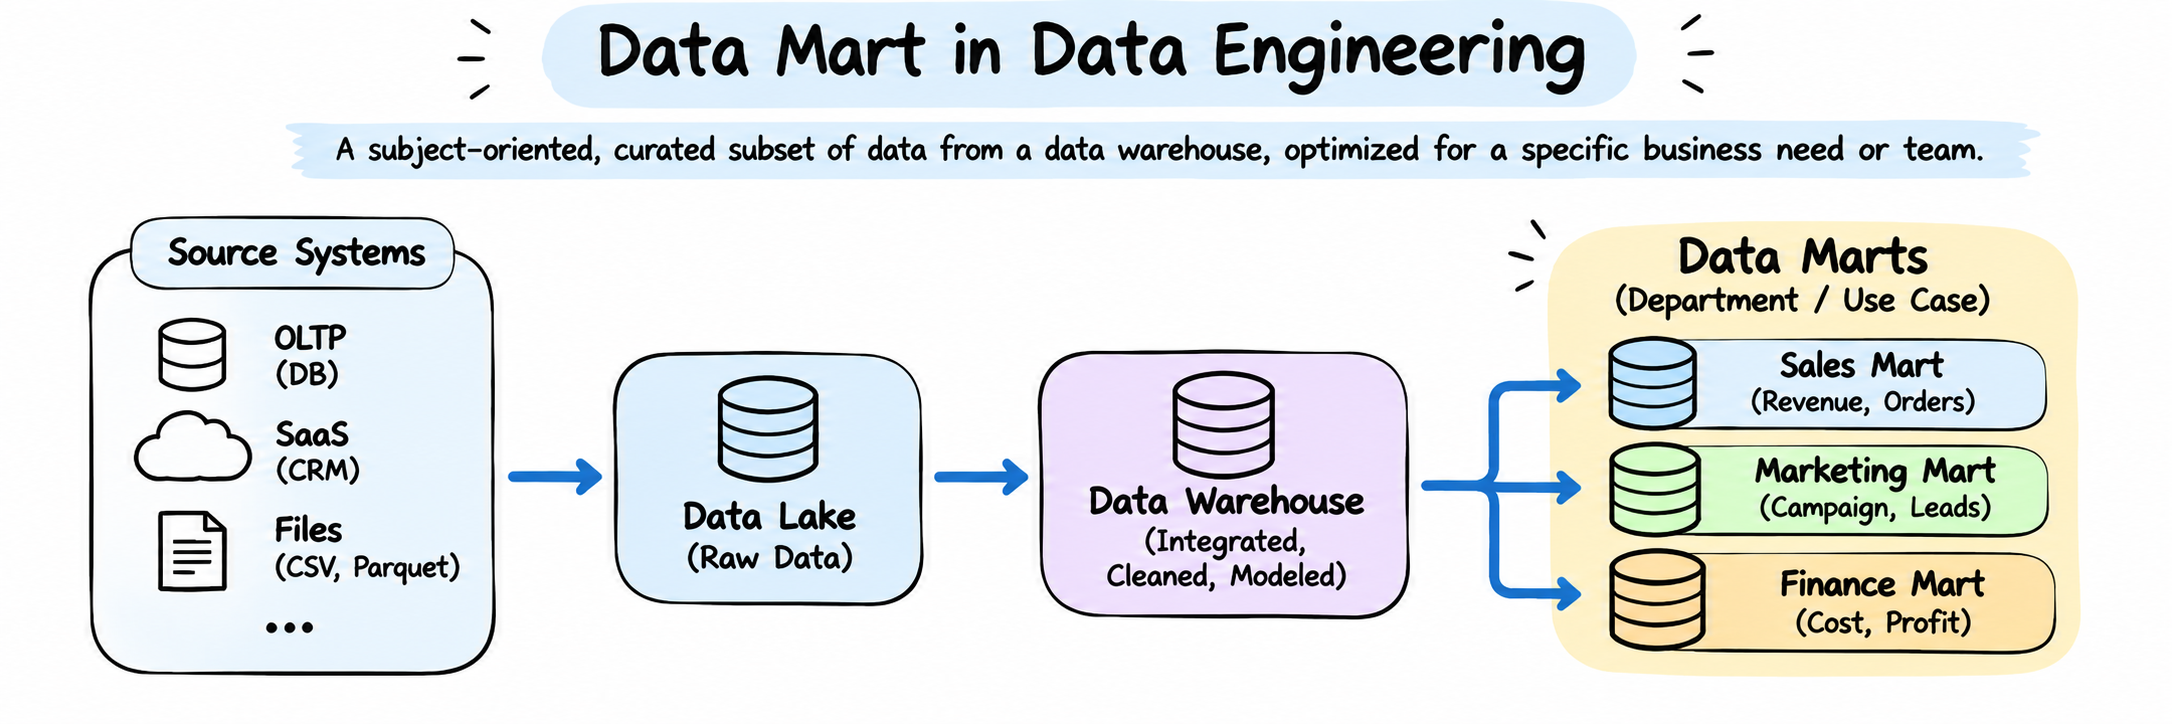
\includegraphics[width=\textwidth]{figures/Data Mart Pipeline Overview.png}
  \caption{Sơ đồ luồng dữ liệu (pipeline) của Data Mart.}
  \label{fig:data-mart-pipeline-overview}
\end{figure}

Vấn đề trên không nằm ở công cụ trực quan hóa (PowerBI, Tableau hay Metabase) mà nằm ở \textbf{tầng kiến trúc dữ liệu phía dưới}: thiếu một nguồn chân lý duy nhất (Single Source of Truth), logic nghiệp vụ bị phân tán ở nhiều nơi và thiếu vắng tầng \textbf{Data Mart} được chuẩn hóa.

Tài liệu này được biên soạn nhằm giúp bạn:
\begin{enumerate}
    \item Hiểu bức tranh tổng quan về công việc của một Data Engineer (Pipelines, Data Modeling, Orchestration).
    \item Nắm vững vai trò của giai đoạn phân tích (Analytics Phase) và lý do Data Mart đóng vai trò sống còn.
    \item Nhìn lại lịch sử tiến hóa kiến trúc (Kimball, Inmon) cho tới các giải pháp hiện đại (OBT, Data Lakehouse, Data Mesh, Semantic Layer).
    \item Phân tích chi tiết cách hiện thực hóa kiến trúc này qua dự án mẫu trong \texttt{draft.md} sử dụng \textbf{dbt} và \textbf{SQL}.
\end{enumerate}

% =============================================================
\section{Outline của tài liệu}

Để có cái nhìn tổng quan trước khi đi vào chi tiết, tài liệu được tổ chức thành 5 phần như sau:

\noindent
\begin{longtable}{@{}>{\RaggedRight\arraybackslash}p{3.1cm}>{\RaggedRight\arraybackslash}p{8.3cm}>{\RaggedRight\arraybackslash}p{4.3cm}@{}}
\rowcolor{rowLavender}
\textbf{Phần} & \textbf{Nội dung} & \textbf{Vấn đề cốt lõi} \\
\addlinespace[3pt]
\endhead

\textbf{1. Bức tranh toàn cảnh về Data Engineering}
& Sứ mệnh của Data Engineer, sự khác biệt giữa OLTP và OLAP, ba trụ cột (Pipelines, Data Modeling, Orchestration) và vị trí của Analytics Phase trong luồng dữ liệu hiện đại.
& Vì sao cần một tầng Transform chuyên biệt \\
\addlinespace[6pt]

\textbf{2. Data Mart: lịch sử và các giải pháp thay thế}
& Định nghĩa Data Mart, cuộc đối đầu Inmon vs. Kimball, và các hướng hiện đại: OBT, Data Lakehouse, Data Mesh, Headless Semantic Layer.
& Tổ chức dữ liệu phục vụ phân tích \\
\addlinespace[6pt]

\textbf{3. dbt và vai trò định hình Data Mart hiện đại}
& Chuyển dịch từ ETL sang ELT, các thực hành Software Engineering mà dbt mang vào dữ liệu, kiến trúc phân tầng Staging $\rightarrow$ Intermediate $\rightarrow$ Marts.
& Chuẩn hóa quy trình Transform \\
\addlinespace[6pt]

\textbf{4. Phân tích thiết kế trong \texttt{draft.md}}
& Macro chống Metric Drift, Intermediate model và khái niệm Grain, hai Data Mart (\texttt{mart\_sales\_daily}, \texttt{mart\_customer\_360}), Semantic Layer và kiểm thử chất lượng dữ liệu.
& Hiện thực hóa Data Mart bằng code \\
\addlinespace[6pt]

\textbf{5. Trade-offs và thảo luận thực tế}
& Chiến lược materialization, khác biệt cú pháp giữa các Cloud Data Warehouse, và thời điểm cần tách Dimension theo chuẩn Kimball (SCD Type 2).
& Đưa thiết kế vào production \\
\end{longtable}

\begin{captionbelowboxaivn}
Bảng 1: Outline 5 phần của tài liệu ``Kiến trúc Data Mart với dbt \& SQL''.
\end{captionbelowboxaivn}

% =============================================================
\section{Bức tranh toàn cảnh về Data Engineering}

\subsection{Sứ mệnh cốt lõi của Kỹ sư Dữ liệu}

Data Engineer chịu trách nhiệm xây dựng và vận hành ``hệ thống đường ống dẫn nước'' cho toàn bộ tổ chức, đảm bảo dữ liệu di chuyển từ nơi phát sinh đến nơi tiêu thụ một cách \textbf{chính xác, kịp thời, an toàn và có thể mở rộng}.

Về bản chất, dữ liệu trong doanh nghiệp chia làm hai thế giới tách biệt:

\noindent
\begin{longtable}{@{}>{\RaggedRight\arraybackslash}p{3.4cm}>{\RaggedRight\arraybackslash}p{4.4cm}>{\RaggedRight\arraybackslash}p{7.6cm}@{}}
\rowcolor{rowLavender}
\textbf{Tiêu chí} & \textbf{OLTP} & \textbf{OLAP} \\
\addlinespace[3pt]
\endhead
Tên đầy đủ & Online Transaction Processing & Online Analytical Processing \\
\addlinespace[3pt]
Hệ thống điển hình & Postgres, MySQL, MongoDB & Snowflake, BigQuery, ClickHouse \\
\addlinespace[3pt]
Mục tiêu tối ưu & Ghi/đọc từng dòng đơn lẻ với độ trễ mili-giây & Quét hàng triệu dòng trên một số cột để tổng hợp (\texttt{SUM}, \texttt{COUNT}, \texttt{AVG}) \\
\addlinespace[3pt]
Thiết kế & Chuẩn hóa (3NF) để tránh trùng lặp khi giao dịch & Phi chuẩn hóa / dimensional để truy vấn nhanh \\
\end{longtable}

\begin{captionbelowboxaivn}
Bảng 2: Hai thế giới dữ liệu OLTP và OLAP.
\end{captionbelowboxaivn}

Để kết nối hai thế giới này, Data Engineer làm việc xoay quanh ba trụ cột:
\begin{enumerate}
    \item \textbf{Data Pipelines (ELT / ETL)}: cơ chế trích xuất dữ liệu từ các nguồn (Operational DBs, Event Streams, 3rd party APIs) và nạp vào Cloud Data Warehouse/Data Lake.
    \item \textbf{Data Modeling}: nghệ thuật tổ chức, làm sạch và định hình lại dữ liệu thô hỗn loạn thành các bảng logic có cấu trúc, phục vụ con người và thuật toán truy vấn.
    \item \textbf{Orchestration}: ``nhạc trưởng'' (Apache Airflow, Dagster, Prefect) quản lý đồ thị phụ thuộc (DAG --- Directed Acyclic Graph), đảm bảo các tác vụ chạy đúng thứ tự, tự động retry khi lỗi, cảnh báo và hỗ trợ chạy bù dữ liệu (backfill).
\end{enumerate}

\subsection{Analytics Phase nằm ở đâu?}

Luồng dữ liệu hiện đại thường đi qua các chặng sau:
\begin{figure}[H]
\centering
\begin{tikzpicture}[node distance=0.55cm, text width=2.3cm]
  \node[dbox] (src) {\textbf{Nguồn}\\[1pt]\footnotesize OLTP, Logs, Events};
  \node[dbox, right=of src] (raw) {\textbf{Raw / Bronze}\\[1pt]\footnotesize Dữ liệu thô trong Warehouse};
  \node[dhi, right=of raw] (tr) {Transform\\[1pt]\footnotesize\mdseries Analytics Phase (dbt)};
  \node[dbox, right=of tr] (mart) {\textbf{Marts / Gold}\\[1pt]\footnotesize Dữ liệu sẵn sàng phân tích};
  \node[dbox, right=of mart] (use) {\textbf{Tiêu thụ}\\[1pt]\footnotesize BI, ML, Apps};
  \draw[darr] (src) -- (raw);
  \draw[darr] (raw) -- (tr);
  \draw[darr] (tr) -- (mart);
  \draw[darr] (mart) -- (use);
  \draw[decorate, decoration={brace, mirror, amplitude=5pt}, color=aivnGreen, thick]
    ([yshift=-0.2cm]raw.south west) -- ($(mart.south east |- raw.south)+(0,-0.2cm)$)
    node[midway, below=9pt, dnote, text width=12cm] {Kho dữ liệu (Warehouse) --- ELT: Load trước, Transform sau};
\end{tikzpicture}
\end{figure}

\begin{figurecaptionmodern}
\capfig{Vị trí của Analytics Phase trong luồng dữ liệu ELT hiện đại.}
\end{figurecaptionmodern}

\begin{infobox}{Analytics Phase là gì?}
Đây chính là giai đoạn \textbf{Transform} trong mô hình \textbf{ELT modern data stack}. Thay vì để nhà phân tích nghiệp vụ hay Data Scientist truy vấn trực tiếp vào bảng thô, Analytics Phase nhận dữ liệu thô đã nạp vào kho, sau đó: (1) làm sạch (loại bản ghi trùng, chuẩn hóa kiểu dữ liệu, đồng nhất timezone); (2) áp dụng business rules (thế nào là đơn hàng hợp lệ? đơn hủy, đơn hoàn tiền tính ra sao?); (3) gom nhóm và tính các chỉ số kinh doanh cốt lõi (KPIs).
\end{infobox}

\subsection{Tại sao cần Analytics Phase chuyên biệt?}

\begin{itemize}
    \item \textbf{Bảo vệ hệ thống và tối ưu chi phí}: một câu query của Data Analyst quét toàn bộ bảng log 500 triệu dòng trên BigQuery trực tiếp từ dashboard có thể tốn hàng trăm USD và làm đơ dashboard. Tầng transform tính sẵn và lưu kết quả giúp dashboard phản hồi tức thì với chi phí tối thiểu.
    \item \textbf{Ngăn chặn ``Logic Drift'' (lệch chuẩn định nghĩa)}: nếu không có tầng transform tập trung, mỗi analyst sẽ tự viết SQL riêng trong công cụ BI. Một người lọc \texttt{status = 'completed'}, người khác lọc \texttt{status IN ('completed', 'shipped')} --- dẫn đến số liệu không bao giờ khớp nhau.
\end{itemize}

% =============================================================
\section{Data Mart: lịch sử, lý do tồn tại và các giải pháp thay thế}

\subsection{Data Mart là gì và tại sao cần Data Mart?}

\begin{infobox}{Định nghĩa}
\textbf{Data Mart} là một tập con của Kho dữ liệu (Data Warehouse), được thiết kế tập trung phục vụ một \textbf{chủ đề nghiệp vụ cụ thể} (subject-oriented) hoặc một phòng ban nhất định (Marketing Mart, Sales Mart, Finance Mart, Customer 360\ldots).
\end{infobox}

Vì sao không để người dùng truy vấn thẳng vào Enterprise Data Warehouse (EDW)?
\begin{itemize}
    \item \textbf{Độ phức tạp}: EDW chứa hàng nghìn bảng liên kết chằng chịt. Người dùng nghiệp vụ hoặc BI developer chỉ cần tập trung vào các thực thể quen thuộc của họ.
    \item \textbf{Hiệu năng \& tối ưu hóa}: Data Mart thường tinh gọn, tiền tổng hợp (pre-aggregated) hoặc phi chuẩn hóa (denormalized) phù hợp đúng loại báo cáo cần hiển thị.
    \item \textbf{Phân quyền \& bảo mật}: dễ dàng cấp quyền để team Marketing chỉ đọc Mart Marketing mà không truy cập được dữ liệu nhạy cảm của HR hay Finance.
\end{itemize}

\subsection{Cuộc đối đầu Inmon vs. Kimball}

Trong hơn 30 năm lịch sử Data Warehousing, có hai trường phái kinh điển:

\begin{aivnplainbox}[Hai trường phái kiến trúc]
[Inmon - Top-Down]
Sources --> Staging --> Normalized 3NF EDW (trung tâm) --> Dependent Data Marts --> BI

[Kimball - Bottom-Up]
Sources --> Staging --> Dimensional Model (Star Schema: Facts + Conformed Dims) --> BI
\end{aivnplainbox}

\noindent
\begin{longtable}{@{}>{\RaggedRight\arraybackslash}p{2.4cm}>{\RaggedRight\arraybackslash}p{6.7cm}>{\RaggedRight\arraybackslash}p{6.7cm}@{}}
\rowcolor{rowLavender}
\textbf{Tiêu chí} & \textbf{Bill Inmon (Top-down)} & \textbf{Ralph Kimball (Bottom-up)} \\
\addlinespace[3pt]
\endhead
\textbf{Triết lý} & Xây dựng EDW chuẩn hóa (3NF) tập trung trước, sau đó tạo các Data Mart phục vụ phòng ban. & Xây các Data Mart theo mô hình Dimensional (Star Schema), liên kết nhau qua Conformed Dimensions (Bus Matrix). \\
\addlinespace[3pt]
\textbf{Ưu điểm} & Tính toàn vẹn cao, tránh dư thừa dữ liệu tối đa. & Triển khai nhanh (time-to-value), thân thiện với người dùng cuối và BI tool. \\
\addlinespace[3pt]
\textbf{Nhược điểm} & Chi phí ban đầu khổng lồ, thời gian hoàn thành kéo dài hàng năm. & Cần kỷ luật cao để giữ tính nhất quán của Conformed Dimensions khi mở rộng. \\
\end{longtable}

\begin{captionbelowboxaivn}
Bảng 3: So sánh Inmon và Kimball.
\end{captionbelowboxaivn}

Suốt nhiều thập kỷ, \textbf{Kimball Dimensional Modeling} (Fact \& Dimension) đã trở thành chuẩn mực thực tế của ngành.

\subsection{Các giải pháp thay thế và hướng phát triển hiện đại}

Hạ tầng lưu trữ và tính toán đám mây đã sinh ra những phương pháp mới thay thế hoặc bổ trợ cho Data Mart truyền thống:

\begin{enumerate}
    \item \textbf{One Big Table (OBT)}: thay vì mô hình sao gồm 1 Fact và 5 Dimension nối nhau qua khóa ngoại, các warehouse dạng cột (BigQuery, ClickHouse, Snowflake) khuyến khích denormalize hoàn toàn thành một bảng duy nhất. \emph{Ưu điểm}: query rất nhanh vì không tốn JOIN, viết đơn giản. \emph{Nhược điểm}: kích thước lưu trữ tăng (dù nén cột giảm thiểu phần nào), dữ liệu bị lặp.
    \item \textbf{Data Lakehouse (Apache Iceberg, Delta Lake)}: xóa nhòa ranh giới giữa Data Lake (rẻ, chứa phi cấu trúc) và Data Warehouse (nhanh, chuẩn ACID). Data Mart ngày nay có thể là các bảng Iceberg được quản lý mở, cho phép nhiều query engine (Trino, Spark, DuckDB) cùng đọc.
    \item \textbf{Data Mesh}: thay vì một team DE trung tâm gánh toàn bộ việc xây Mart cho cả công ty, quyền sở hữu dữ liệu chuyển giao cho các domain team (ví dụ domain Order sở hữu pipeline và Data Product Order). Data Mart trở thành một \textbf{Data Product} có SLA rõ ràng.
    \item \textbf{Headless Semantic Layer (dbt Semantic Layer, Cube.js)}: thay vì nhét mọi phép tổng hợp vào các bảng vật lý tĩnh, ta định nghĩa logic tính toán trong một tầng metadata chung. Tầng này nhận yêu cầu từ Tableau hay PowerBI và tự sinh SQL tối ưu đẩy xuống warehouse xử lý.
\end{enumerate}

\begin{figure}[H]
\centering
\begin{tikzpicture}[text width=2.6cm]
  \node[dind] (k) at (0,0)     {\textbf{Kimball}\\[1pt]\footnotesize Star Schema, Conformed Dims};
  \node[dbox] (o) at (3.4,0)   {\textbf{OBT}\\[1pt]\footnotesize Một bảng phi chuẩn hóa, không JOIN};
  \node[dbox] (l) at (6.8,0)   {\textbf{Lakehouse}\\[1pt]\footnotesize Iceberg / Delta, nhiều engine cùng đọc};
  \node[dbox] (s) at (10.2,0)  {\textbf{Semantic Layer}\\[1pt]\footnotesize Metric định nghĩa một lần, sinh SQL};
  \node[dblue] (m) at (13.6,0) {\textbf{Data Mesh}\\[1pt]\footnotesize Domain sở hữu Data Product};
  \node[dnote, above=0.15cm of k] {chuẩn hóa mô hình};
  \node[dnote, above=0.15cm of o] {tối ưu truy vấn};
  \node[dnote, above=0.15cm of l] {hạ tầng lưu trữ mở};
  \node[dnote, above=0.15cm of s] {logic chỉ số};
  \node[dnote, above=0.15cm of m] {tổ chức \& sở hữu};
  \draw[{Stealth[length=2.5mm]}-{Stealth[length=2.5mm]}, thick, color=gray!70]
    (-1.3,-1.6) -- (14.9,-1.6);
  \node[dnote, anchor=west, text width=4cm] at (-1.3,-2.0) {Tập trung hóa};
  \node[dnote, anchor=east, text width=4cm, align=right] at (14.9,-2.0) {Phi tập trung hóa};
\end{tikzpicture}
\end{figure}

\begin{figurecaptionmodern}
\capfig{Bản đồ các hướng tiếp cận tổ chức dữ liệu phân tích.}
\end{figurecaptionmodern}

% =============================================================
\section{dbt và vai trò định hình Data Mart hiện đại}

\subsection{Cuộc cách mạng từ ETL sang ELT}

Trước đây, công cụ ETL (Informatica, Talend, SSIS) phải tự tính toán trên server riêng rồi mới nạp vào kho. Với sức mạnh tính toán song song khổng lồ của Cloud Data Warehouse, trật tự đảo ngược: \textbf{Extract \& Load toàn bộ dữ liệu thô vào kho trước, sau đó dùng chính sức mạnh của kho để Transform (ELT)}.

\textbf{dbt (data build tool)} trở thành tiêu chuẩn vàng cho chữ \textbf{T} trong ELT, mang các thực hành tốt nhất của Software Engineering vào Data Engineering:
\begin{itemize}
    \item \textbf{Version Control}: mọi model dữ liệu là code SQL lưu trên Git.
    \item \textbf{Module hóa \& quản lý phụ thuộc}: hàm \texttt{\{\{ ref('model\_name') \}\}} giúp dbt tự biên dịch thành DAG hoàn chỉnh, không cần hard-code tên database hay schema.
    \item \textbf{Automated Testing}: viết test như unit test để đảm bảo dữ liệu không NULL, không trùng lặp và thỏa mãn các ràng buộc logic.
    \item \textbf{CI/CD}: tự động test dữ liệu trên môi trường staging trước khi merge vào production.
\end{itemize}

\subsection{Kiến trúc phân tầng kinh điển trong dbt}

Một dự án dbt chuẩn chia mã nguồn thành ba tầng rõ rệt:

\noindent
\begin{longtable}{@{}>{\RaggedRight\arraybackslash}p{3.6cm}>{\RaggedRight\arraybackslash}p{12.2cm}@{}}
\rowcolor{rowLavender}
\textbf{Tầng} & \textbf{Vai trò} \\
\addlinespace[3pt]
\endhead
\textbf{Staging} (\texttt{stg\_}) & Làm sạch kỹ thuật: đổi tên cột, ép kiểu, quan hệ 1:1 với bảng nguồn. \\
\addlinespace[3pt]
\textbf{Intermediate} (\texttt{int\_}) & Single Source of Truth: JOIN các thực thể, xử lý logic phức tạp. \\
\addlinespace[3pt]
\textbf{Marts} (\texttt{mart\_}) & Tầng phục vụ: Fact, Dimension, bảng tổng hợp theo business domain. \\
\end{longtable}

\begin{captionbelowboxaivn}
Bảng 4: Ba tầng của một dự án dbt chuẩn (Sources $\rightarrow$ Staging $\rightarrow$ Intermediate $\rightarrow$ Marts).
\end{captionbelowboxaivn}

\begin{figure}[H]
\centering
\begin{tikzpicture}[node distance=0.7cm]
  \node[dbox, text width=3.4cm] (src) {\textbf{Sources (Raw)}};
  \node[dbox, text width=3.4cm, below=of src] (stg) {\textbf{Staging} \texttt{stg\_}};
  \node[dbox, text width=3.4cm, below=of stg] (int) {\textbf{Intermediate} \texttt{int\_}};
  \node[dhi, text width=3.4cm, below=of int] (mart) {Marts \texttt{mart\_}};
  \draw[darr] (src) -- (stg);
  \draw[darr] (stg) -- (int);
  \draw[darr] (int) -- (mart);
  \node[right=0.6cm of src, anchor=west, font=\small, text width=10.5cm] {Bảng thô do pipeline Extract \& Load nạp vào kho};
  \node[right=0.6cm of stg, anchor=west, font=\small, text width=10.5cm] {Làm sạch kỹ thuật: đổi tên cột, ép kiểu, quan hệ 1:1 với nguồn};
  \node[right=0.6cm of int, anchor=west, font=\small, text width=10.5cm] {Single Source of Truth: JOIN các thực thể, áp dụng business logic, xác định grain};
  \node[right=0.6cm of mart, anchor=west, font=\small, text width=10.5cm] {Tầng phục vụ: Fact, Dimension, bảng tổng hợp theo business domain};
\end{tikzpicture}
\end{figure}

\begin{figurecaptionmodern}
\capfig{Kiến trúc phân tầng trong một dự án dbt.}
\end{figurecaptionmodern}

% =============================================================
\section{Phân tích thiết kế trong \texttt{draft.md}}

Bản thảo \texttt{draft.md} cung cấp một ví dụ mẫu mực về cách xây dựng Data Mart phục vụ dashboard cho ngành thương mại điện tử (E-commerce). Dưới đây là phân tích từng thành phần.

\subsection{Macro: chốt chặn duy nhất chống ``Metric Drift''}

\begin{aivnplainbox}[macros/business\_logic.sql]
{% macro revenue_expr() %}
    CASE
        WHEN o.order_status = 'completed'
        THEN (oli.quantity * oli.unit_price * (1 - oli.discount_pct))
             - COALESCE(oli.refund_amount, 0)
        ELSE 0
    END
{% endmacro %}

{% macro is_valid_order() %}
    o.order_status IN ('completed', 'shipped')
    AND o.is_test_order = FALSE
{% endmacro %}
\end{aivnplainbox}

\begin{itemize}
    \item \textbf{Vấn đề}: ``Doanh thu'' là khái niệm dễ gây tranh cãi nhất. Có tính đơn đang giao (shipped) không? Đơn hoàn tiền có trừ ra không? Chiết khấu tính thế nào? Có loại tài khoản test của nhân viên QA không?
    \item \textbf{Giải pháp}: dbt Macro đóng gói toàn bộ logic này thành một hàm Jinja tái sử dụng. Mọi model cần tính doanh thu hoặc lọc đơn hợp lệ \textbf{bắt buộc} gọi \texttt{\{\{ revenue\_expr() \}\}} và \texttt{\{\{ is\_valid\_order() \}\}}. Khi định nghĩa nghiệp vụ thay đổi, kỹ sư dữ liệu \textbf{chỉ cần sửa đúng một chỗ}.
\end{itemize}

\subsection{Intermediate model: nguồn chân lý duy nhất}

\begin{aivnsqlbox}[models/intermediate/int\_order\_lines\_enriched.sql]
SELECT
    o.order_id,
    o.customer_id,
    o.order_date,
    o.order_status,
    oli.product_id,
    oli.quantity,
    oli.unit_price,
    oli.discount_pct,
    oli.refund_amount,
    c.customer_segment,
    c.acquisition_channel,
    c.first_order_date,
    {{ revenue_expr() }}  AS net_revenue
FROM {{ ref('stg_orders') }} o
JOIN {{ ref('stg_order_items') }} oli USING (order_id)
JOIN {{ ref('stg_customers') }} c USING (customer_id)
WHERE {{ is_valid_order() }}
\end{aivnsqlbox}

\begin{infobox}{Khái niệm then chốt: Grain}
\textbf{Grain} (độ mịn của dữ liệu) của model này là \textbf{từng dòng sản phẩm trong đơn hàng} (\texttt{order\_id} + \texttt{product\_id}). Đây là độ mịn sâu nhất có thể; từ đó ta tổng hợp lên cấp đơn hàng, khách hàng, hoặc ngày/tháng mà không mất thông tin.
\end{infobox}

\textbf{Tính tái sử dụng}: bằng cách gom sẵn thông tin khách hàng (\texttt{customer\_segment}, \texttt{acquisition\_channel}) và tính sẵn \texttt{net\_revenue} tại đây, các tầng Mart phía sau không phải viết lại các câu JOIN lặp đi lặp lại.

\subsection{Hai Data Mart chuyên biệt}

\subsubsection{Mart 1: Hiệu suất bán hàng theo ngày}

\begin{itemize}
    \item \textbf{File}: \texttt{models/marts/sales/mart\_sales\_daily.sql}
    \item \textbf{Đối tượng phục vụ}: Ban giám đốc (C-level), Trưởng phòng Sales.
    \item \textbf{Grain}: cấp độ ngày (\texttt{order\_date}).
\end{itemize}

Kỹ thuật SQL đáng chú ý:

\begin{aivnsqlbox}[Tính tỷ lệ an toàn với NULLIF]
SUM(net_revenue) / NULLIF(COUNT(DISTINCT order_id), 0) AS avg_order_value,
SUM(refund_amount) / NULLIF(SUM(net_revenue), 0)       AS refund_rate
\end{aivnsqlbox}

\begin{notebox}
\textbf{Xử lý lỗi chia cho 0}: luôn dùng \texttt{NULLIF(..., 0)} cho mẫu số khi tính tỷ lệ (AOV, Refund Rate) để pipeline không sập khi gặp ngày không có đơn hàng.
\end{notebox}

\subsubsection{Mart 2: Khách hàng 360 \& Giữ chân}

\begin{itemize}
    \item \textbf{File}: \texttt{models/marts/customer/mart\_customer\_360.sql}
    \item \textbf{Đối tượng phục vụ}: đội ngũ CRM, Marketing, Chăm sóc khách hàng.
    \item \textbf{Grain}: từng khách hàng duy nhất (\texttt{customer\_id}).
\end{itemize}

Các chỉ số hành vi và phân nhóm (segmentation):
\begin{itemize}
    \item \textbf{Customer Lifetime Value (LTV)}: \texttt{SUM(net\_revenue)} trên toàn bộ vòng đời.
    \item \textbf{Customer Tier}: phân loại mức độ gắn bó (\texttt{one\_time}, \texttt{repeat}, \texttt{loyal}) dựa trên số lượng đơn.
    \item \textbf{Heuristic Churn Risk}: cảnh báo khách đã ngừng mua sắm quá 90 ngày để Marketing kích hoạt chiến dịch re-engagement.
\end{itemize}

\begin{aivnsqlbox}[Cờ nguy cơ rời bỏ (cú pháp BigQuery)]
last_order_date < DATE_SUB(CURRENT_DATE(), INTERVAL 90 DAY) AS is_churn_risk
\end{aivnsqlbox}

\begin{figure}[H]
\centering
\begin{tikzpicture}[text width=5.6cm]
  \node[dind, text width=7cm] (int) at (0,0) {\texttt{int\_order\_lines\_enriched}\\[1pt]\footnotesize Grain: từng dòng sản phẩm trong đơn};
  \node[dhi, text width=6.2cm] (a) at (-4.4,-3) {\texttt{mart\_sales\_daily}};
  \node[dhi, text width=6.2cm] (b) at (4.4,-3) {\texttt{mart\_customer\_360}};
  \draw[darr] (int.south) -- ++(0,-0.6) -| node[pos=0.25, above, dnote] {\texttt{GROUP BY order\_date}} (a.north);
  \draw[darr] (int.south) -- ++(0,-0.6) -| node[pos=0.25, above, dnote] {\texttt{GROUP BY customer\_id}} (b.north);
  \node[dbox, below=0.5cm of a, text width=6.2cm, font=\footnotesize] {Grain: ngày\\Phục vụ: C-level, Trưởng phòng Sales\\AOV, Refund Rate};
  \node[dbox, below=0.5cm of b, text width=6.2cm, font=\footnotesize] {Grain: khách hàng\\Phục vụ: CRM, Marketing, CSKH\\LTV, Tier, Churn Risk};
\end{tikzpicture}
\end{figure}

\begin{figurecaptionmodern}
\capfig{Từ một Intermediate model sinh ra hai Data Mart với grain khác nhau.}
\end{figurecaptionmodern}

\subsection{Tách tầng ngữ nghĩa (Semantic Layer) khỏi Dashboard}

\begin{aivnplainbox}[mart\_sales\_daily.yml]
semantic_models:
  - name: sales
    model: ref('mart_sales_daily')
    entities:
      - name: date
        type: time
        expr: order_date
    measures:
      - name: net_revenue
        agg: sum
      - name: total_orders
        agg: sum

metrics:
  - name: average_order_value
    type: ratio
    label: AOV
    type_params:
      numerator: net_revenue
      denominator: total_orders
\end{aivnplainbox}

\textbf{Tại sao không để công cụ BI tự tính AOV?} Nếu để BI tự tính, người tạo biểu đồ có thể vô tình lấy \texttt{AVG(net\_revenue)} thay vì \texttt{SUM(net\_revenue) / COUNT(order\_id)} --- hai con số hoàn toàn khác nhau. Khi khai báo thước đo cơ bản (\texttt{measures}) và công thức tỷ lệ (\texttt{metrics}) trong dbt Semantic Layer, BI tool chỉ còn đóng vai trò \textbf{tầng hiển thị} (presentation layer).

\subsection{Đảm bảo chất lượng dữ liệu bằng kiểm thử}

\begin{aivnplainbox}[Data tests trong schema.yml]
models:
  - name: mart_sales_daily
    tests:
      - dbt_utils.equal_rowcount:
          compare_model: ref('int_order_lines_enriched')
    columns:
      - name: net_revenue
        tests:
          - not_null
          - dbt_utils.expression_is_true:
              expression: ">= 0"
\end{aivnplainbox}

\begin{itemize}
    \item \textbf{Chặn dữ liệu bất thường}: đảm bảo doanh thu ròng không bao giờ âm (trừ khi có nghiệp vụ đặc thù).
    \item \textbf{Đối soát số lượng dòng (row-count reconciliation)}: phát hiện ngay nếu phép JOIN làm ``nở'' dữ liệu (Cartesian product / fan-out bug) gây sai lệch toàn bộ số liệu báo cáo.
\end{itemize}

% =============================================================
\section{Trade-offs và thảo luận thực tế}

Khi đưa thiết kế trong \texttt{draft.md} vào production, kỹ sư dữ liệu cần cân nhắc ba vấn đề lớn sau.

\subsection{Chiến lược materialization}

\noindent
\begin{longtable}{@{}>{\RaggedRight\arraybackslash}p{2.4cm}>{\RaggedRight\arraybackslash}p{7.2cm}>{\RaggedRight\arraybackslash}p{6.2cm}@{}}
\rowcolor{rowLavender}
\textbf{Loại} & \textbf{Đặc điểm} & \textbf{Phù hợp} \\
\addlinespace[3pt]
\endhead
\texttt{view} & Không tốn dung lượng, luôn mới nhất, nhưng query chậm nếu bảng nguồn lớn. & Tầng Staging \\
\addlinespace[3pt]
\texttt{table} & Tốn dung lượng và thời gian build, nhưng dashboard query cực nhanh. & Mart phục vụ dashboard hằng ngày \\
\addlinespace[3pt]
\texttt{incremental} & Chỉ xử lý và chèn dữ liệu phát sinh từ lần chạy trước (ví dụ ngày hôm qua). & Bắt buộc khi bảng đơn hàng chạm mốc hàng chục triệu dòng \\
\end{longtable}

\begin{captionbelowboxaivn}
Bảng 5: Các chiến lược materialization trong dbt.
\end{captionbelowboxaivn}

\subsection{Khác biệt cú pháp giữa các Cloud Data Warehouse}

Hàm xử lý ngày tháng trong \texttt{draft.md} đang dùng cú pháp của Google BigQuery. Cùng một logic sẽ được viết khác đi trên các nền tảng khác:

\noindent
\begin{longtable}{@{}>{\RaggedRight\arraybackslash}p{2.8cm}>{\RaggedRight\arraybackslash}p{6.3cm}>{\RaggedRight\arraybackslash}p{6.7cm}@{}}
\rowcolor{rowLavender}
\textbf{Nền tảng} & \textbf{Chênh lệch ngày} & \textbf{Lùi 90 ngày} \\
\addlinespace[3pt]
\endhead
BigQuery & \texttt{DATE\_DIFF(MAX(order\_date), MIN(order\_date), DAY)} & \texttt{DATE\_SUB(CURRENT\_DATE(), INTERVAL 90 DAY)} \\
\addlinespace[3pt]
Snowflake & \texttt{DATEDIFF('day', MIN(order\_date), MAX(order\_date))} & \texttt{DATEADD('day', -90, CURRENT\_DATE())} \\
\addlinespace[3pt]
PostgreSQL / Redshift & \texttt{MAX(order\_date) - MIN(order\_date)} & \texttt{CURRENT\_DATE - INTERVAL '90 days'} \\
\end{longtable}

\begin{captionbelowboxaivn}
Bảng 6: Cú pháp xử lý ngày tháng giữa các Cloud Data Warehouse.
\end{captionbelowboxaivn}

\begin{guidelinebox}{Khuyến nghị}
Dùng package \texttt{dbt\_date} hoặc các hàm cross-database như \texttt{dbt.dateadd} để code chạy xuyên suốt trên mọi nền tảng, tránh bị khóa chặt (lock-in) vào một warehouse.
\end{guidelinebox}

\subsection{Khi nào cần tách Dimension theo chuẩn Kimball?}

Hiện tại \texttt{mart\_customer\_360} vừa đóng vai trò Dimension khách hàng, vừa chứa các chỉ số tổng hợp (Aggregated Fact). Thiết kế dạng bảng rộng (Wide Table) này rất trực quan và tiện lợi cho dashboard CRM.

Tuy nhiên, nếu quy mô dữ liệu mở rộng lớn và có nhu cầu \textbf{theo dõi lịch sử thay đổi thông tin khách hàng} (đổi địa chỉ, đổi hạng thành viên), chúng ta cần triển khai thêm kỹ thuật \textbf{Slowly Changing Dimensions (SCD Type 2)} của Kimball --- chủ đề của tài liệu tiếp theo.

% =============================================================
\section{Tổng kết}

Thiết kế dữ liệu không chỉ là viết các câu lệnh SQL để ra con số, mà là một \textbf{quy trình kỹ thuật có hệ thống}:
\begin{enumerate}
    \item Đảm bảo dữ liệu chảy mượt mà từ hệ thống nguồn qua các đường ống được điều phối chặt chẽ.
    \item Chuẩn hóa và làm sạch tại tầng Intermediate với grain xác định.
    \item Tập trung hóa logic tính toán chỉ số bằng macro và Semantic Layer để loại bỏ tình trạng sai lệch số liệu.
    \item Đóng gói thành các Data Mart chuyên biệt, tối ưu hiệu năng cho người dùng cuối và dashboard.
\end{enumerate}

\end{document}
